\subsection{The Larger Scope of Applicability}
\label{sec:analysis1:larger_context_of_applicability}
Determining the results above, we set focus on discovering missing abstract operations. Therefore, we ignore documents and service operations if openISBT does not support them for other reasons than undiscovered abstract operations. Figure \ref{fig:analysis1_pie_both_criteria_all_factors} visualizes the metrics as figure \ref{fig:analysis1_pie_both_criteria_main} but reflects any aspect of applicability.

\begin{figure}[!hb]
\centering
\begin{subfigure}[t]{.48\textwidth}
  \centering
%%%%%%%%%%%%%%%%%%%%%%%%%%%%%%%%%%%%%%%%%%% 
%%%%%%%%%%%%%%% OPERATIONS %%%%%%%%%%%%%%%%
%%%%%%%%%%%%%%%%%%%%%%%%%%%%%%%%%%%%%%%%%%% 
    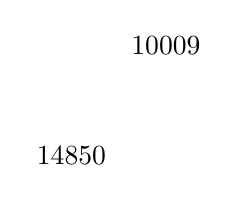
\begin{tikzpicture}
        \pie[ 
            /tikz/every pin/.style={align=left},
            sum=auto,
            radius=2,
            text=pin,
            rotate=120,
            before number=\phantom,
            after number=,
            color={red!70,blue!70}
            ]{
            14.850/$\textbf{Not supported}$\\ (59.7\%),
            10.009/$\textbf{Supported}$\\ (40.3\%)
            };
            \node[] at (0.6, 0.7){10009};
            \node[] at (-0.6,-0.7){14850};
    \end{tikzpicture}
%%%%%%%%%%%%%%%%%%%%%%%%%%%%%%%%%%%%%%%%%%% 
%%%%%%%%%%%%%%%%%%%%%%%%%%%%%%%%%%%%%%%%%%% 
%%%%%%%%%%%%%%%%%%%%%%%%%%%%%%%%%%%%%%%%%%% 
  \caption{OpenISBT matches 10009 of 24859 Operations across all APIs.}
  \label{fig:analysis1_sub_pie_coverage_sup_operations_all_factors}
\end{subfigure}%
\hfill
\begin{subfigure}[t]{.48\textwidth}
  \centering
%%%%%%%%%%%%%%%%%%%%%%%%%%%%%%%%%%%%%%%%%%% 
%%%%%%%%%%%%%%%%%% APIs %%%%%%%%%%%%%%%%%%%
%%%%%%%%%%%%%%%%%%%%%%%%%%%%%%%%%%%%%%%%%%% 
    \begin{tikzpicture}
        \pie[ 
            /tikz/every pin/.style={align=left},
            sum=auto,
            radius=2,
            text=pin,
            rotate=90,
            % before number=\phantom,
            % after number=,
            color={red!70,blue!70}
            ]{
            1159/$\textbf{Not fully}$ \\$\textbf{supported}$ \\ (75.6\%),
            375/$\textbf{Fully supported}$\\ (24.4\%)
            }
    \end{tikzpicture}
%%%%%%%%%%%%%%%%%%%%%%%%%%%%%%%%%%%%%%%%%%% 
%%%%%%%%%%%%%%%%%%%%%%%%%%%%%%%%%%%%%%%%%%% 
%%%%%%%%%%%%%%%%%%%%%%%%%%%%%%%%%%%%%%%%%%% 
  \caption{For 375 of 1534 APIs openISBT matches all operations.}
  \label{fig:analysis1_sub_pie_coverage_full_sup_apis_all_factors}
\end{subfigure}%
\caption{Coverage metrics for a set of 1534 OpenAPI documents including 24859 service operations}
\label{fig:analysis1_pie_both_criteria_all_factors}
\end{figure}


Therefore, it considers 1534 OpenAPI documents, which define 24859 service operations on top-level resources and nested resources.
If openISBT cannot process an OpenAPI document without exception, or the OpenAPI document only defines nested resources, we count it as $p_i=0$. Figure  \ref{fig:analysis1_sub_pie_coverage_sup_operations_all_factors} shows a  much smaller coverage of 40.3\% for the supported service operations.
Also, figure \ref{fig:analysis1_sub_pie_coverage_full_sup_apis_all_factors} shows a smaller coverage of 24.4\% for the fully supported APIs. 
